\documentclass[11pt]{article}

\usepackage[margin=1in]{geometry}
\usepackage{tikz}
\usepackage[strict]{changepage}
\usepackage{amsthm}
\usepackage{float}
\usepackage{fancyhdr}
 
\theoremstyle{definition}
\newtheorem{definition}{Definition}[section]

\title{ESE 370: Project 2 Final Report}

\author{Pranav Kunapuli and Martin Deng}

\date{\today}

\pagestyle{fancy}
\fancyhf{}
\rhead{Pranav Kunapuli and Martin Deng}
\lhead{ESE 370: Project 2 Final Report}
\cfoot{\thepage}

\begin{document}

\begin{enumerate}

\item \textbf{Schematics}\\

\begin{figure} [H]
	\caption{SRAM Memory Cell Schematic}
    \centering
    	\includegraphics[scale=0.5]{SRAM_Schematic.png}
\end{figure}

\begin{figure} [H]
	\caption{Basic Cell Test Schematic}
    \centering
    	\includegraphics[scale=0.5]{Basic_Cell_Read_Write_Stable.png}
\end{figure}

\begin{figure} [H]
	\caption{Basic Cell with Tristate Configuration Schematic}
    \centering
    	\includegraphics[scale=0.5] {Basic_Cell_Read_Write_Tristate.png}
\end{figure}

\begin{figure} [H]
	\caption{Column Driver Schematic}
    \centering
    	\includegraphics[scale=0.5]{Column_Driver.png}
\end{figure}

\begin{figure} [H]
	\caption{Column Precharger Schematic}
    \centering
    	\includegraphics[scale=0.5]{Column_Precharger.png}
\end{figure}

\begin{figure} [H]
	\caption{Sense Amp Schematic}
    \centering
    	\includegraphics[scale=0.5]{Sense_Amp.png}
\end{figure}

\begin{figure} [H]
	\caption{Tristate Buffer Schematic}
    \centering
    	\includegraphics[scale=0.5]{Tri_Buffer.png}
\end{figure}

\item \textbf{Enqueue and Dequeue Operations} \\

\item \textbf{Memory Operation and Design Choices} \\
We'll start with an explanation of our memory cell. As we stated in our milestone, we began by designing an SRAM memory cell of minimum size, and we tested our read and write operations with a 20ps period clock signal. 

\begin{enumerate}

\item \textbf{Demonstration of Writing to Cell} \\
\begin{figure} [H]
	\caption{Unamplified Bit Line Voltages}
    \centering
    	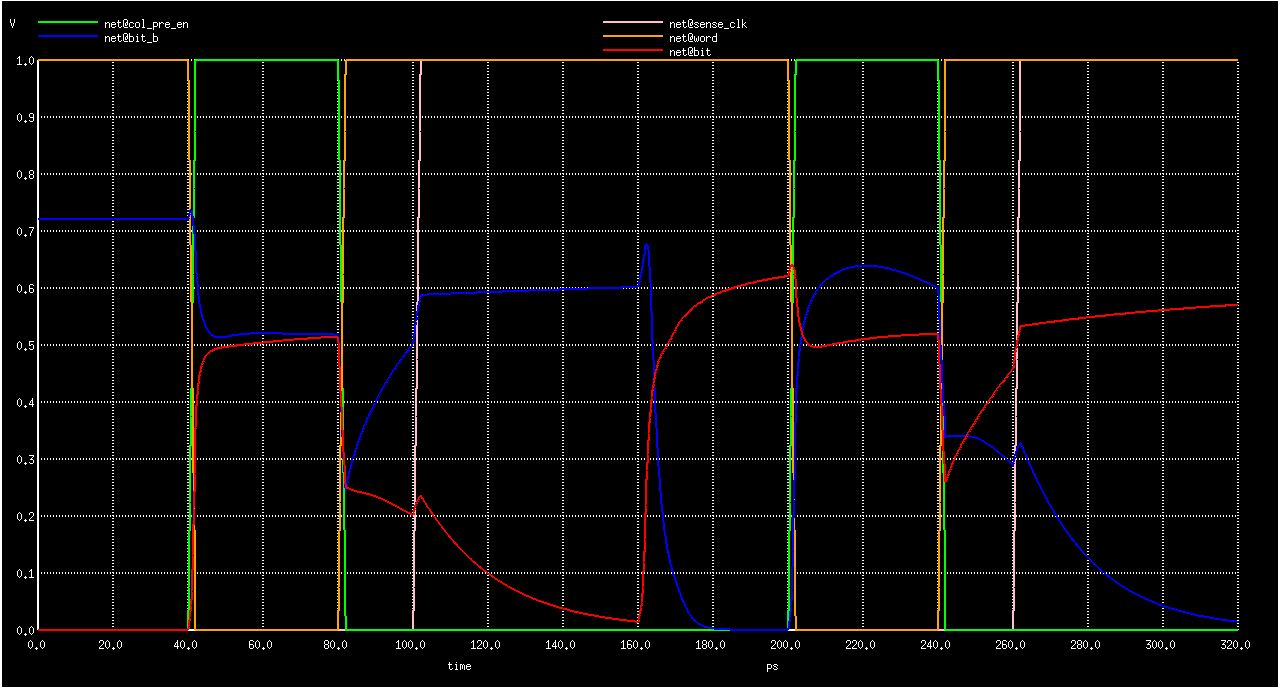
\includegraphics[scale=0.4]{basic_cell_read_write_raw.JPG}
\end{figure}

\begin{figure} [H]
	\caption{Amplified Bit Line Voltages}
    \centering
    	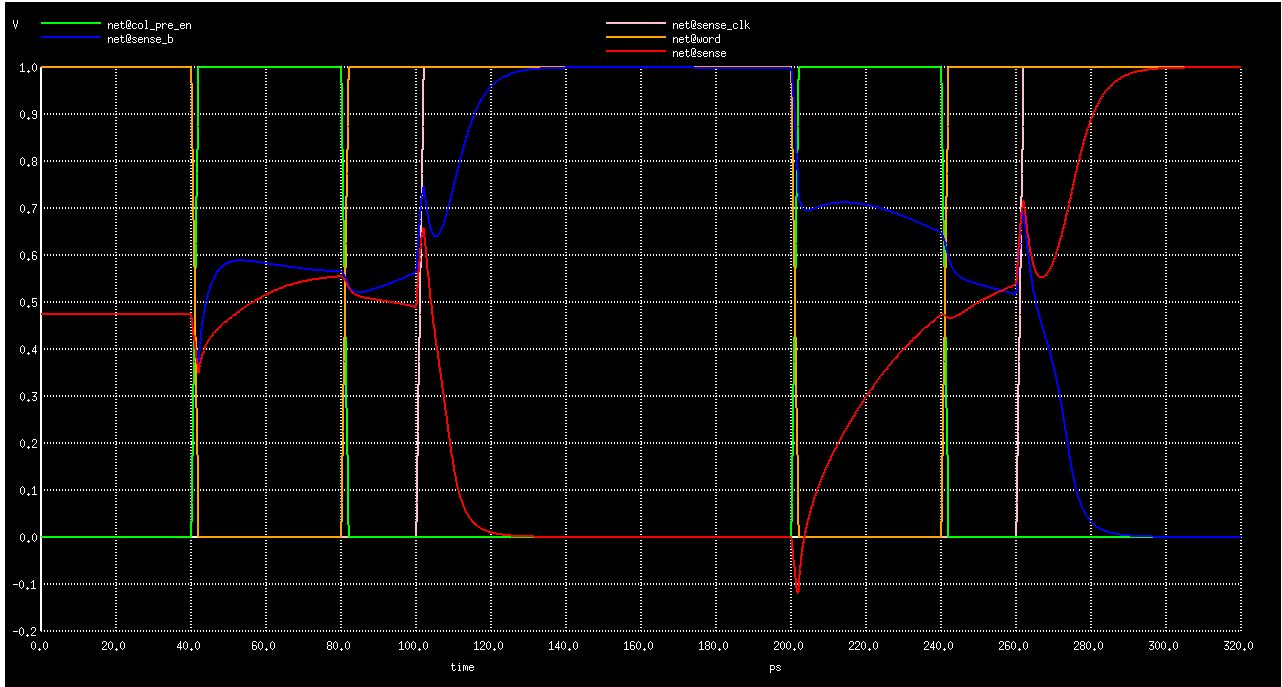
\includegraphics[scale=0.4]{basic_cell_read_write_restored.JPG}
\end{figure}

We see from these two graphs that our write function performs exactly as expected. Let us first take a look at our unamplified graph. We see around 80 ps that our word line goes high, and we are initially trying to write low to our memory cell. At the 80 ps mark, the word line switches, and we see that shortly after, our bit line goes to almost 0 V and our bit-b line goes to around 0.6 V. This shows that we can properly write low to the cell. Then again at 240 ps, we see the second instance of our word line going high, but this time we are trying to write high to our memory cell. After this instance, we see that our bit line goes to 0.6 V and our bit-b line goes to 0 V. Thus we can write both low and high to our memory cell. We were also able to reverse the order of writing high and low to satisfy all four of our test conditions, and those writes were also successful.

Now we can turn our attention to Figure 9. Here, we see the same behavior as in Figure 8, except we see both the bit line and the bit-b line being driven to rail. This demonstrates the functionality of our sense amplifier. It picked up that there was a minor change on the two lines and then drives the two lines to rail.

\item \textbf{Demonstration of Reading from Cell} \\
\begin{figure} [H]
	\caption{Reading High from Memory Cell}
    \centering
    	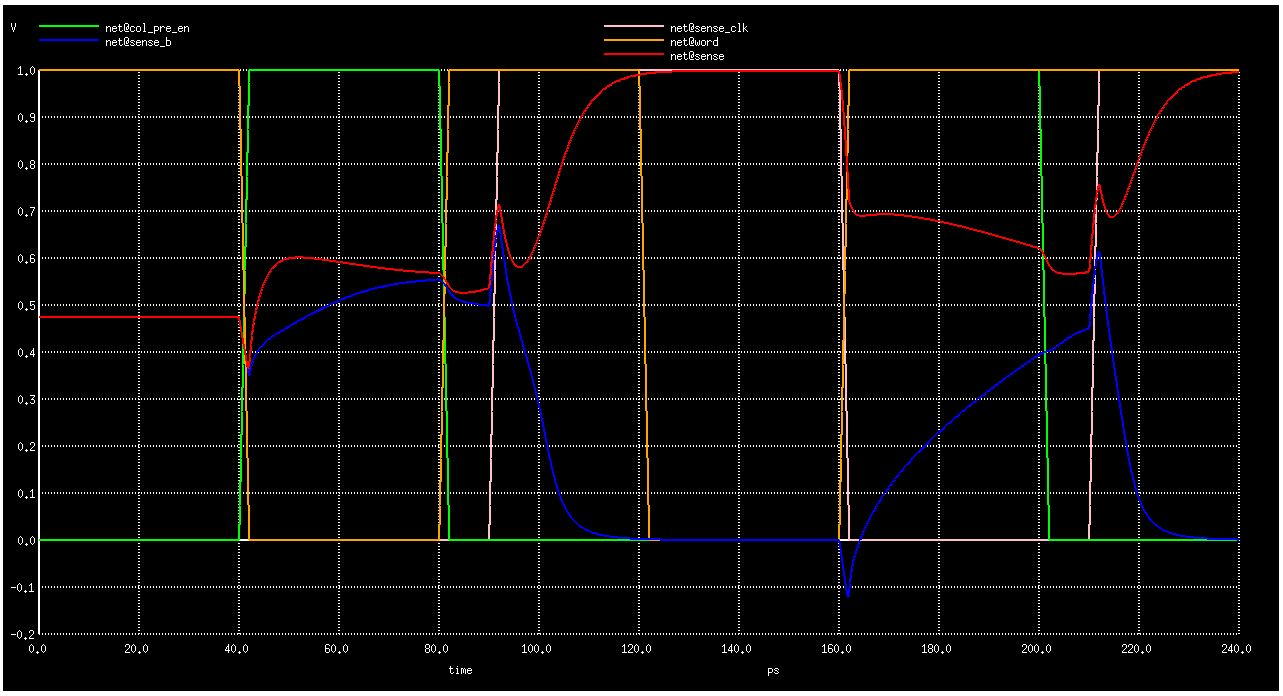
\includegraphics[scale=0.4]{basic_cell_read_stability_one_restored.JPG}
\end{figure}

\begin{figure} [H]
	\caption{Reading Low from Memory Cell}
    \centering
    	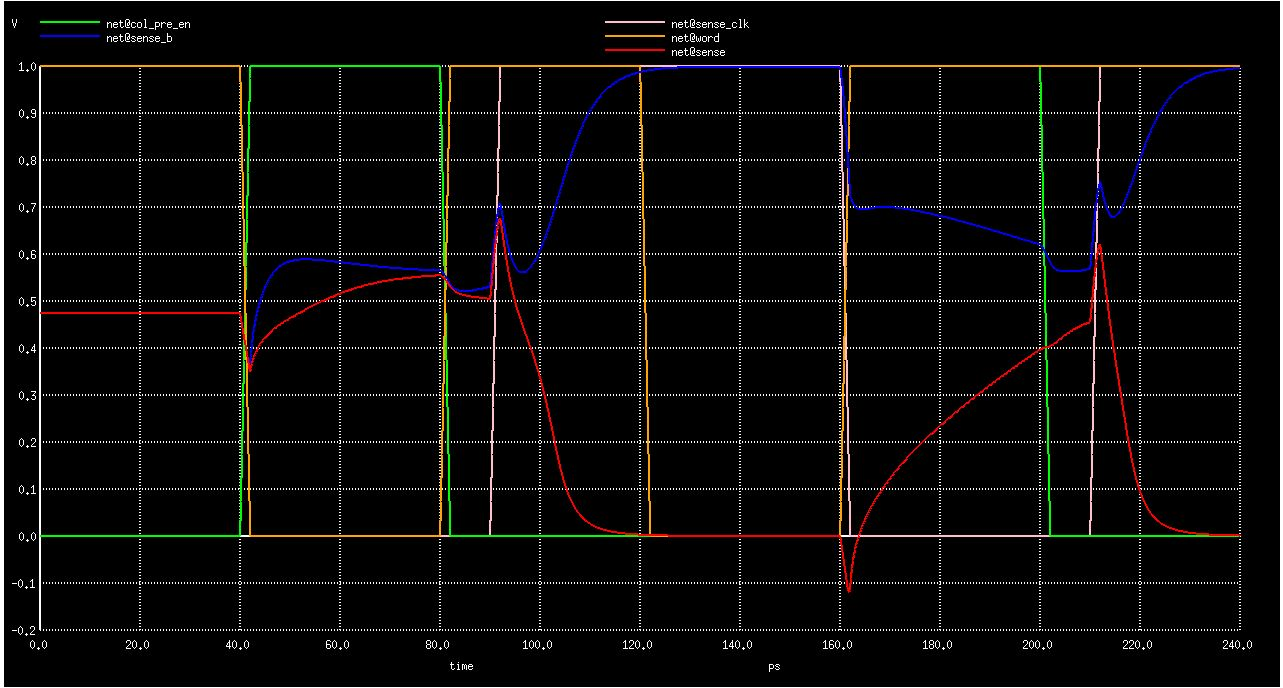
\includegraphics[scale=0.4]{basic_cell_read_stability_zero_restored.JPG}
\end{figure}

These two test cases are very similar to our write cases. At around 80 ps the word line goes high, indicating that we are ready to perform a read operation. At around 90 ps, the sense clock goes high, which activates our sense amplifier. From 90 ps to the next rising edge of the word line (approximately 160 ps) and the sense clock (approximately 210 ps), we see that the value that we are reading is held strong at rail for both the bit line and the bit-b line. The only differences between the two simulations is whether the bit line goes high or low, which depends on whether we are reading a high value from the memory cell or a low value. 

\end{enumerate}

Based on these two operations, we found that our memory cell worked as expected within a 20-30ps time frame. These tests also showed us that we could size our SRAM cell at minimum size, as the time it takes for us to read and write would fit well within the time constraints of a 500 MHz clock. 

From here, for the rest of the milestone, we began working on a few things, including our V-ref circuit, which allows us to operate the entire circuit at half voltage (provided to us), and we created a column driver to charge our bit and bit-b lines. We also created a sense amplifier that could detect changes in our bit and bit-b line signals and amplify them to rail. 

After these milestone modules, we began to create registers or flip-flops to hold some values within the circuit. We started by creating d latches, and then cascading our d-latches to create a register. One of the obvious uses of these registers is for our input and output signals. As our inputs come in (i.e. in[3:0], enqueue, and dequeue), we first pass them into a register. We also latch our outputs (i.e. full, empty, out[3:0]) to a registers at the end. All of this is done so that we can make sure our circuit operates correctly given certain inputs and clock signals. We wouldn't want to be in a situation where we are in the middle of a write or read operation and our signals switch on us, causing us to abandon the operation mid way, thereby giving us incorrect operation. Next we will explain how our timing works to remedy this potential problem.

Given a clock signal, on the rising edge, we take all inputs and throw them into input registers, and we take all output signals and update the output registers as well. Then, while the clock remains high, we use the time to precharge our bit and bit-b lines and word lines based on our new inputs. When the clock goes low, we take a small chunk of time first to perform a read operation, after which we spend the rest of the low clock time writing in new values. Then again, when we get a rising clock edge, we again put all inputs and outputs in registers, and repeat the process.

One thing that had to get done for this portion of the project was to correctly store `head and tail pointers'. That is to say, we needed to know which row to read from and where to write to in our array of memory cells. The way we do this is through our shift-register module. 

First, we must explain an invariant of our system. We chose to define `empty' as when our read and write pointers were at the same row, and our `full' signal was when the read pointer was one higher than the write pointer. That too, the way we work a write operation is that we first update the pointer and then we write, but for reading, we first read and then we update the pointer. This leads to a discrepancy of two slots in the queue, which actually presents a new issue. In order to use this functionality, we had to add two extra rows to our memory cells, making 10 rows instead of 8. But although there are 10 rows, we still only store a maximum of 8 elements at a time.

Now that we have explained this invariant, we can explain the operation of our word line selectors. This module works by setting the zeroth word line as high and every other word line as low at the start. Then, on every clock cycle, as long as the enable signal was high and the stack signal was low (we will explain these two signals shortly), the values in the register would shift. Because the eighth, or last, register in our shift register circuit was linked to the first, no new inputs could be introduced. Only the single high signal can be rotated through the 9 registers. This rotation works differently for the write and read operations. For the write operation, the enable signal is the enqueue signal, and the stack signal is the full output signal. So when we want to enqueue and the queue isn't full, we move on to the next word line. For the read operation, the enable signal is the dequeue signal, and the stack signal is the empty output signal. 

The empty and full output signals also have their own tester modules. As we said earlier, the empty signal is turned on if the same word line is pointed to by both the read shift registers and the write shift registers. The full signal is turned on if the write pointer is ever one less than the read pointer. For example, if we are trying to read from word line 0 and trying to write to word line 8, we know we already have 8 elements, so the full signal turns on and writing is disabled. 

The last module we have to cover is our bit driver module. The bit driver takes in our bit and bit-b lines and switches between reading and writing during the low clock signal period. 

\item \textbf{Energy Breakdown}\\

\item \textbf{Energy Optimization}\\

\item \textbf{Design Validation and Test Cases}\\
We began design validation with our memory cell, using the circuit in Figure 3. We used this circuit to validate that we could properly read and write to a single memory cell. This circuit, as stated earlier, also validated operation of our column driver and our sense amp. We used the test cases of reading and writing both low and high values, as well as reading and writing based on different starting states. 

From there, we then proceeded to test our different modules that we created after our milestone. We first tested our word line drivers and our full and empty testers by running a clock signal through them and checking that on appropriate inputs, the word lines would switch, and whenever the full or empty signals were high, either the write or read word lines would stop switching respectively. After testing the testers and the word line drivers, we then tested the bit driver, which routes the bit lines to perform a read operation or a write operation. We tested this by feeding a delayed clock into the bit driver. While the original clock is low and delayed clock is high, we perform a read, but when that delayed clock is low and the original clock is low, we switch to writing until the original clock goes high.

\item \textbf{Design Metrics}\\

\begin{enumerate}

\item \textbf{Memory Cell Area}\\
We found back in our milestone that we were able to size our SRAM memory cell at minimum size and still get correct operation even with a 20ps test clock cycle. Figure 1 shows our memory cell, and we see that each transistor is minimum sized, for a total memory cell area of 6. Because we have 8 rows of memory cells, each containing 4 cells to hold 4-bit values, we have a total area for all of the 32 memory cells of 192. 

\item \textbf{Area}\\
Here is the area breakdown for each of our modules:

\begin{center}
\begin{tabular} { | c || c | }
	\hline
    Module & Area \\
    \hline
    Inverter & 4 \\
    NAND2 & 4 \\
    NOR2 & 4 \\
    NAND3 & 6 \\
    NOR3 & 6 \\
    SRAM & 6 \\
    Memory Array & 192 \\
    Bit Driver & 42 \\
    Clock Delay & 20 \\
    Column Driver & 36 \\
    Column Precharge & 88 \\
    D Register & 24 \\
    Word Line Driver & 230 \\
    Empty Tester & 72 \\
    Full Tester & 72 \\
    IO Registers & 144 \\
    Sense Amp & 10 \\
    FIFO & 1320 \\
    \hline
\end{tabular}
\end{center}


\item \textbf{Enqueue Energy}\\
We found that the integral of the enqueue current came to 0.35 pA, which means our enqueue energy came to 0.35 pJ given an operating voltage of 1V. This was for the scenario of enqueue-ing 0x1111 to a cell that previously held 0x0000.

\item \textbf{Dequeue Energy}\\
We found that the integral of the enqueue current came to 0.33 pA, which means our enqueue energy came to 0.33 pJ given an operating voltage of 1V. This was for the scenario of dequeue-ing 0x0000. 

\item \textbf{Enqueue/Dequeue Energy}\\
When both enqueue-ing and dequeue-ing in the same cycle, we found our energy to be 0.37 pJ. This is because based on our design, both the read and the write operation occur at the same time, and so our energy for both is limited. This is the scenario of writing 0x1111 to a cell that previously had 0x0000 and reading 0x0000 when the output was previously 0x1111.

\item \textbf{Standby Energy}\\
In the standby case, the energy came to be 0.34 pJ. 

\item \textbf{Average Energy}\\
In the case of having 15\% enqueue&dequeue, 10\% enqueue, 10\% dequeue, and 65\% standby operation, the total energy came out to just 0.34 pJ.

\end{enumerate}

\begin{center}
I, \textbf{Pranav Kunapuli}, certify that I have complied with the \\
University of Pennsylvania’s Code of Academic Integrity \\
in completing this project
\end{center}

\begin{center}
I, \textbf{Martin Deng}, certify that I have complied with the \\
University of Pennsylvania’s Code of Academic Integrity \\
in completing this project
\end{center}

\end{enumerate}

\end{document}